\textbf{Autor: Anil, Tugce}

\glqq{}Grade+\grqq{} ist ein Terminplanungssystem für mündliche Prüfungen. In das System können sich Personen anmelden, wobei es vier unterschiedliche vordefinierte Rollen (Prüfer, Student, StudentExaminer und Admin) gibt. Die Unterscheidung wird maßgeblich durch unterschiedliche Zugriffsberechtigungen deutlich, aber auch Attribute können sich unterscheiden. Das folgende UML Modell soll die Datenstruktur dabei deutlicher machen. Im folgenden soll das Modell außerdem durch Betrachtung einzelner Teile des Datenmodells detaillierter Beschrieben werden.
\begin{figure}[H]
	\centering
  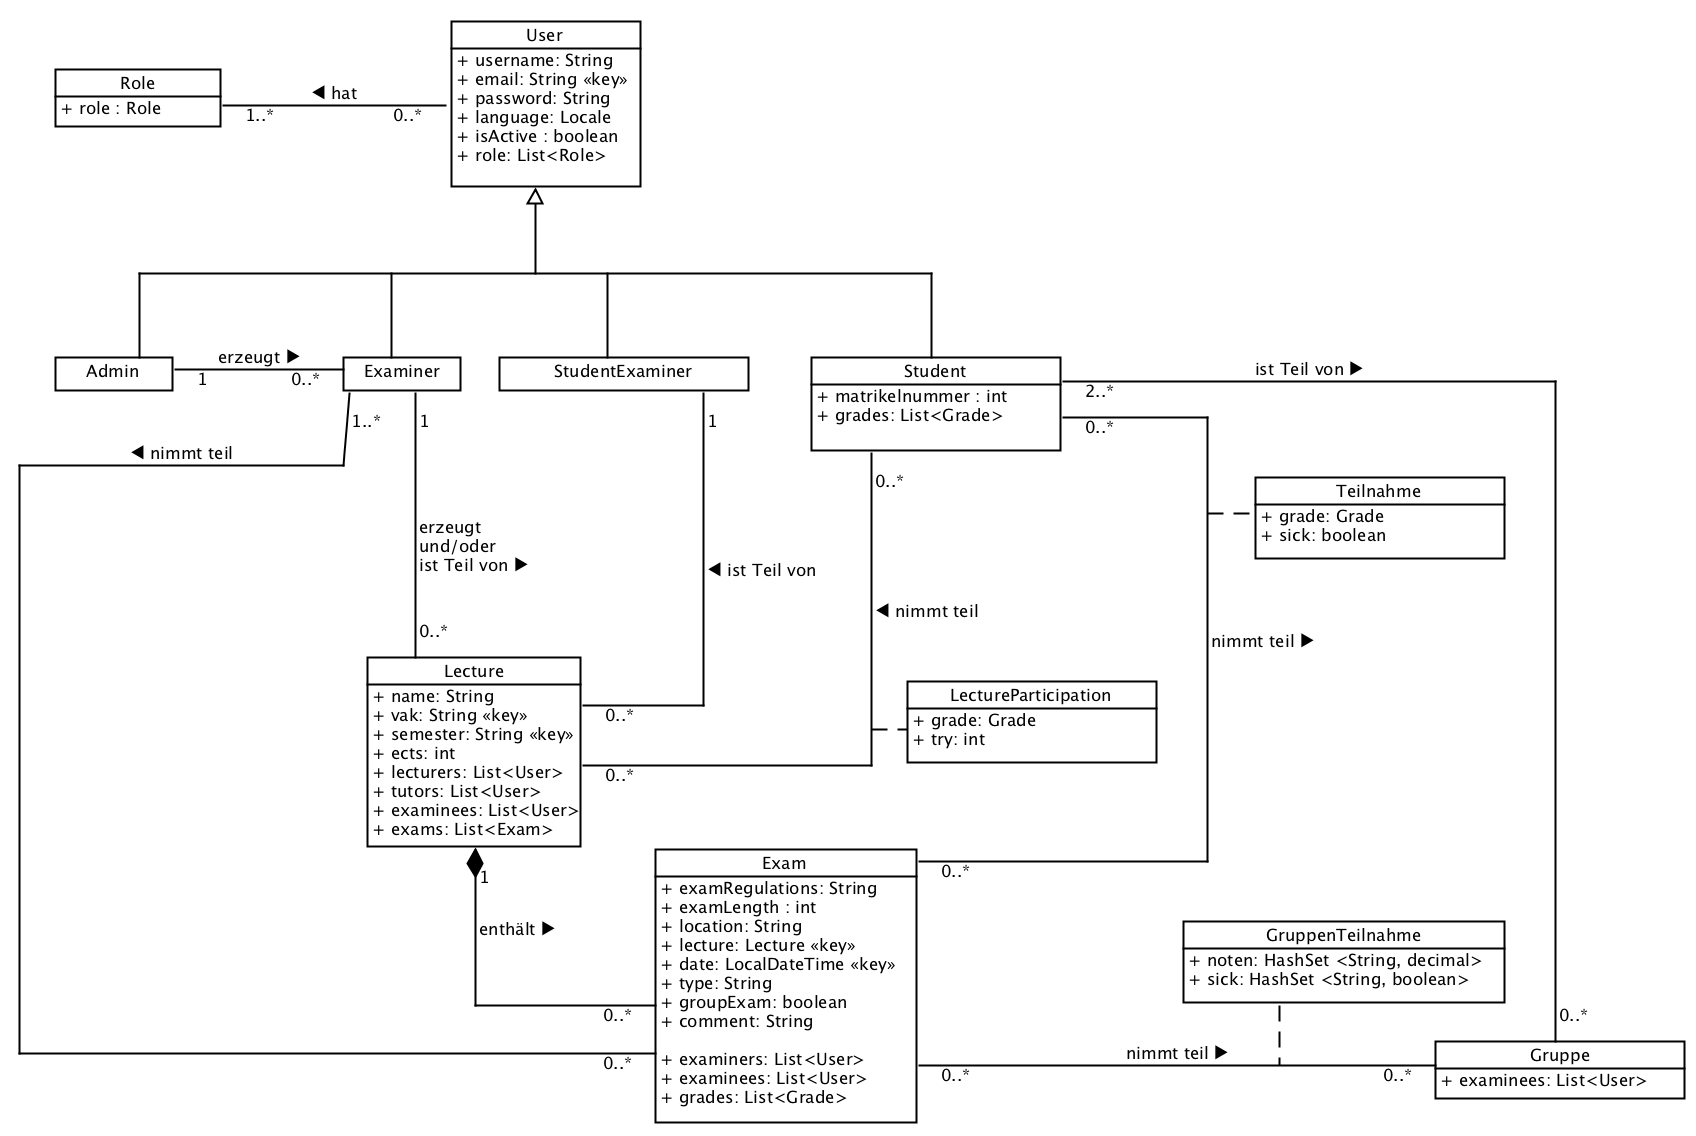
\includegraphics[width=\textwidth,height=10cm,keepaspectratio]{../UMLDiagramme/datenmodell/alles.png}
	\caption{Datenmodell als UML-Klassendiagramm}
	\label{fig 0}
\end{figure}


\subsubsection{User}
\begin{figure}[H]
	\centering
  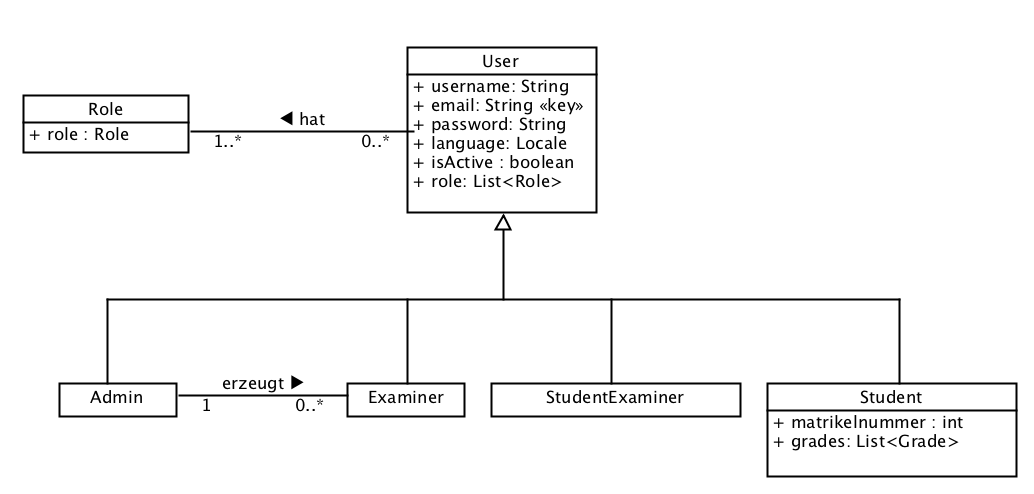
\includegraphics[width=\textwidth,height=10cm,keepaspectratio]{../UMLDiagramme/datenmodell/user.png}
	\caption{Users als UML-Klassendiagramm}
	\label{fig 1}
\end{figure}
Admin, Examiner und Student sind verschiedene User, die alle von der Oberklasse User erben.
Die verschiedenen Rollen sind in der Klasse Role definiert. Ein Student, der in Prüfungen (Exam) als Prüfer teilnimmt, bekommt zusätzlich zur Rolle „Student“ noch die Rolle
StudentExaminer.
Alle User werden durch ihre e-mail eindeutig bestimmt. 
In der Datentabelle wird der Unterschied der User durch die unterschiedliche Rollenverteilung deutlich. Dabei kann ein User mehrere Rollen übernehmen.
Das Attribut isActive gibt an, ob das Konto gibt an, ob das Konto des Users aktiv ist oder deaktiviert wurde.
Wenn ein User die Rolle Student hat der User zusätzlich noch eine Martrikelnummer und eine Liste von Noten.

\subsubsection{Examiner und StudentExaminer}
\begin{figure}[H]
	\centering
  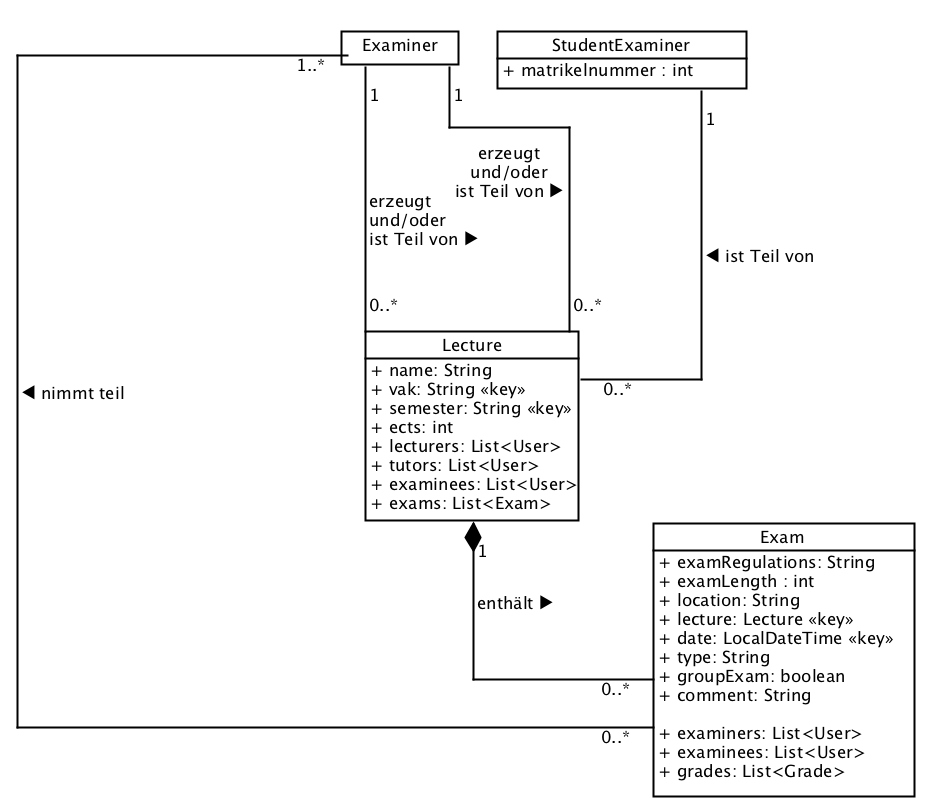
\includegraphics[width=\textwidth,height=10cm,keepaspectratio]{../UMLDiagramme/datenmodell/examiner.png}
	\caption{Examiner und StudentExaminer als UML-Klassendiagramm}
	\label{fig 2}
\end{figure}
Nur der Examiner (Prüfer) kann eine Lehrveranstaltung (Lecture) erzeugen. 
Examiner und StudentExaminer können an einer Lehrveranstaltung teilnehmen.
Eine Lehrveranstaltung kann mehrere Exam (Prüfungstermine) erhalten.
Durch das Startdatum und die zugehörige Lehrveranstaltung kann ein Exam eindeutig bestimmt werden.


\subsubsection{Student}
\begin{figure}[H]
	\centering
  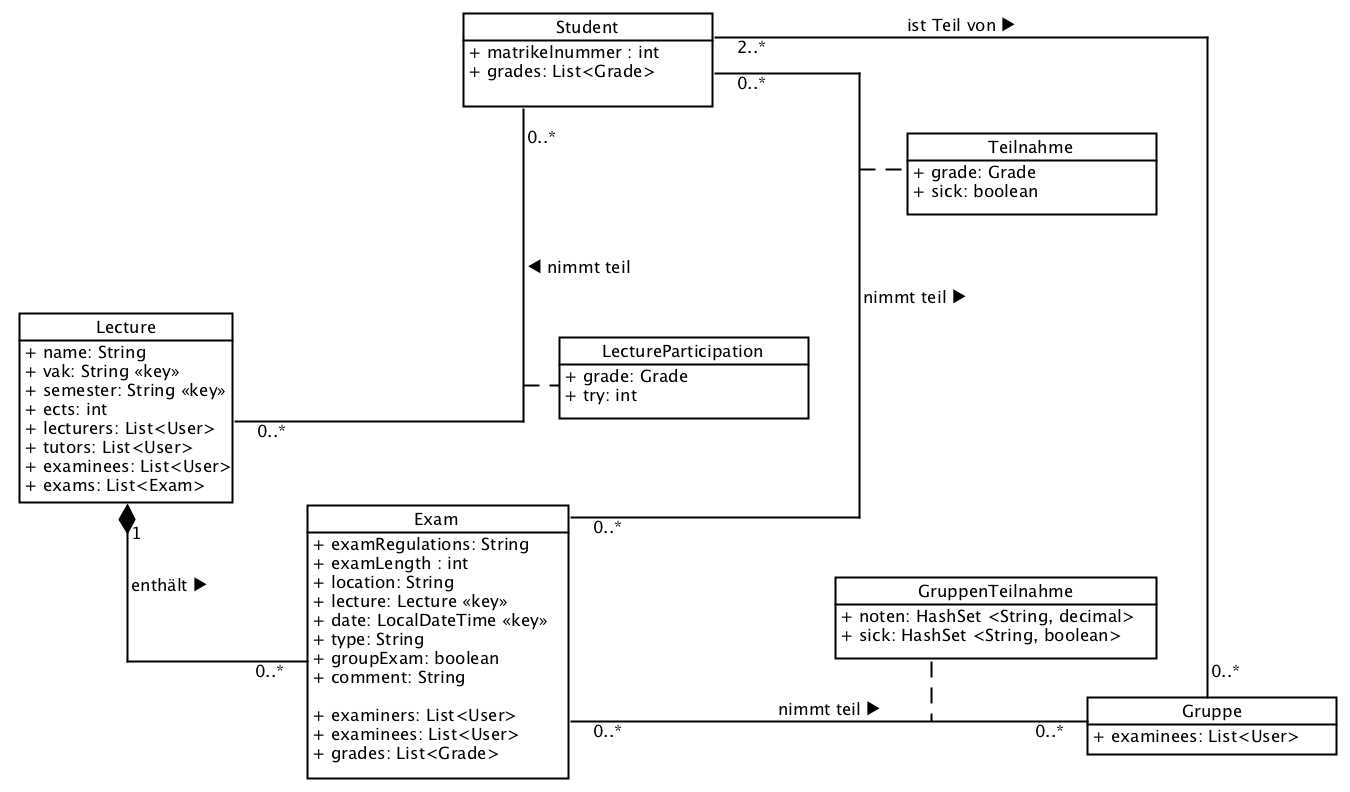
\includegraphics[width=\textwidth,height=10cm,keepaspectratio]{../UMLDiagramme/datenmodell/student.png}
	\caption{Student als UML-Klassendiagramm}
	\label{fig 3}
\end{figure}
Ein Student kann in einer Lehrveranstaltung eingeschrieben sein. Durch die Teilnahme an der Lehrveranstaltung erhält der Student eine Note und Prüfungsversuche für die Lehrveranstaltung. Ein Student kann immer einzeln oder als Gruppe an einer Klausur teilnehmen.

\subsection{Anwendung der Strategien auf die Datensicht}
Es wurden alle Entscheidungen und Strategien (\ref{K5}) aus den vorherigen Sichten, auch in der Datensicht berücksichtigt.
\\
\textbf{S16: Mehrsprachigkeit:}\\
Die Spracheinstellungen des Nutzers werden in dem Datenschema User (siehe \ref{fig 1}) abgespeichert. Dadurch kann die Srachpräferenz eines jeden Nutzers gespeichert werden.\\
\textbf{S17: Benachrichtigung der Nutzer:}\\
Jeder Nutzer ist in der Datenbank mitsamt seiner E-Mail-Adresse eingetragen. Die Benachrichtigungen werden an eben diese E-Mail-Adressen geschickt.\\
\textbf{S19: Nutzer-Verwaltung:}\\
Das Programm wird alle Daten die in dem Datenmodell genannt werden für die entsprechenden Nutzer langfristig speichern.
Außerdem wurden alle Relationen aus dem Datenmodell in die Software übernommen.\\
\textbf{S24: Daten-Backup erzeugen:}\\
Das Daten-Backup wird das Datenmodell abbilden und ein Spiegelbild der Datenbank zum Erstellungszeitpunkt des Backups sein.  